\section{Networking, Localization, and Data Management Framework for Drone}
\label{networkingsection}
%Navigation, networking, localization

For autonomous drone-based monitoring, the prerequisite is a self-operating framework.
Two crucial factors that need to be considered for autonomous operation is speed, and safety. Beside data management is another important factor.

\subsection{Autonomous Navigation}
In the known environment, a drone can avoid obstacles easily. While in an unknown environment, it is difficult to operate. In the majority case, either the system is safe but slow, or the system works fast but unsafe. In very recent research a system has been implemented that can operate independently in an unknown environment safely, with a good speed. The real world with drone's perspective can be divided into two parts; the flying zone of the drone and the outside map area. A map with a drone's perspective is shown in Fig~\ref{autonomous}. They have partitioned the flying zone area into 3 spaces~\cite{tordesillas2019real, tordesillas2019faster}. The first one is known free space (F) which is the instructed space with no construction change. The second space is known but occupied space (O) which can be represented by the change in construction or the intervene of any real-world object such as a bird. And the last one is the unknown space (U) that might be required based on the real-world situation.
\begin{figure}[h!]
\centering
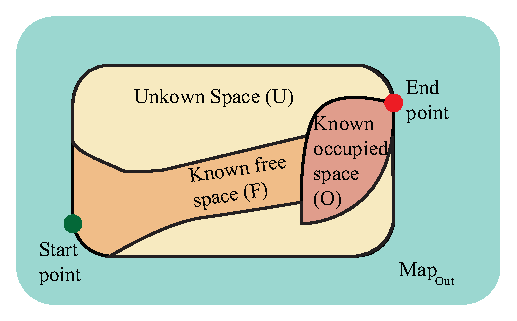
\includegraphics[width=.8\linewidth]{figure/autonomous.eps}
\caption{Flying map with drone perspective.}
\label{autonomous}
\end{figure}

In the proposed system by the authors in~\cite{liu2017planning}, Jump Point Search (JPS) is used as an universal planner to find the shortest possible route from the starting point to the ending point~\cite{harabor2011online}. Another alternative technique is A\(^*\) search but JPS not only ensures faster magnitude but also guarantees the completeness and optimality. This hierarchical input control consists of three parts i.e., a part controlled by jerk, a part controlled by velocity, and a part controlled by geometry. By using the map, the collision search for each of the three primitives shown above the whole performance can be summarized as follows. If it does not collide, the jerk operated trajectory is treated as collision-free. The velocity-controlled primitive is forced to traverse the JPS solution's paths. Eventually, a no-hit obstacle is confirmed to hit the JPS route. 
% The cost for the planned trajectory is calculated by the following equations.
% $$\text{Cost}=J_{\text{Prim}_{j}}+J_{\text{Prim}_{v}}+J_{\text{Prim}_{d}}$$

% Here, $J_{\text{Prim}_{j}}$ represents jerk-controlled primitive, $J_{\text{Prim}_{v}}$ is combination of multiple primitives regulated by velocity, and $J_{\text{Prim}_{d}}$ is the portion of JPS.

Besides, a monocular camera based drone system was proposed, where can operate autonomously in the preceding unknown indoor hallway area, where GPS is not working properly~\cite{padhy2018deep}. They have used the CNN model to reach the goal. Video captured by the camera is fed to the model, then the model takes the decision. The CNN model is designed with 4 convolutional layers and 4 pooling layers. The output of the model is left, right, and straight.

A deep learning-based network was experimented on a little shaped drone, where the drone was able to navigate autonomously in many different circumstances, e.g., a  relatively straight forest trail with 100 m length, a  zigzag forest path with 6 turns, a 1 km mountainous zigzag forest path, and an open field~\cite{smolyanskiy2017toward}. The network namely TrailNet is inspired by sResNet-18. SResNet-18 is basically a ResNet-18 with batch normalization and shifted Relu function is used instead of Relu fucntion \cite{he2016deep}. Input of the TrailNet is the image capured by the drone and outputs of the model are view orientation and lateral offset. By using these two output parameters the drone can fly indepnedently. Besides, they have also implemented safety feature for the drone, e.g., obstacle detection and avoidance.

In the racing track, a drone have to pass though several square gates. As all the gates look exactly same, and one gate is visiable through others, it is a very diffcullt task to dected the nearest gate.A ADRNet (Autonoumous Drone Racing Network) was developed for this purpose~\cite{jung2018perception}. ADRNet  is a CNN based network. Using this network and line-of-sight guidance algorithm they developed a drone system, that can comeplete a race track. 

\subsection{Safety Features}
In practical life, a drone may encounter unexpected obstacles such as a ball coming toward it, which can cause damage to the drone. Besides, covering 360$^{\circ}$ safety is not only costly but also computation expensive too. Therefore, one possible solution is using sonar sensors embedded with the drone. One of the possible solutions is utilizing the Doppler effect~\cite{garg2020enabling}. According to the formula, a drone can detect Doppler shift for a nearby moving obstacle coming towards the drone with $v_{\circ}$ speed and an $\theta$ angle with the drone then the doppler shift will be, $$\Delta f=f_{\circ} \frac{2 v_{\circ} \cos (\theta)}{v}$$ 


%if a sound source with $f_{\circ}$ coming towards an object with a $v_s$ velocity, then the frequency experienced by the object will be $$f=f_{\circ} \frac{v+v_{s}}{v-v_{t}}$$

% Here, $v$ and $v_t$ are the speed of sound and target respectively. However, with a stationary sound source and microphone system as shown in Fig~\ref{safety}, a drone can detect Doppler shift for a nearby moving obstacle coming towards the drone with $v_{\circ}$ speed. According to the theorem, the total Droppler shift will be, $$\Delta f=f_{\circ} \frac{2 v_{\circ}}{v-v_{\circ}}\approx f \frac{2 v_{\circ}}{v} \left[\text{as } v_{\circ}<<v\right]$$

\begin{figure}[h!]
\centering
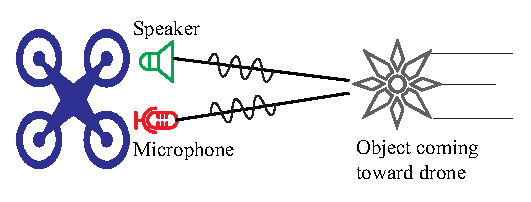
\includegraphics[width=.8\linewidth]{figure/safety.eps}
\caption{Doppler effect on drone.}
\label{safety}
\end{figure}

% Considering the velocity direction, if the moving object makes an $\theta$ angle with the drone, then only the cosine component of the object's velocity will influence the doppler shift. On that case, $$\Delta f=f_{\circ} \frac{2 v_{\circ} \cos (\theta)}{v}$$ 

A stationary sound source and microphone system as shown in Fig~\ref{safety}, a drone can detect Doppler shift for a nearby moving obstacle coming towards the drone with $v_{\circ}$ speed. However in practice, the doppler shift deviates from the ideal value because of various factors such as environmental drag. Therefore, instead of estimating the Doppler effect, the change of the effect is calculated with respect to $\Delta $ time. As $v_{\circ}$ and $\theta$ are both functions of time, the ratio will be, $$\frac{\Delta f(t+\Delta t)}{\Delta f(t)} \approx \frac{\cos \left[ \theta(t+\Delta t)\right]}{\cos \left[\theta(t)\right]}$$

This angle ratio is the changing rate of radial angle. If the value is constantly one over multiple time segments, then it means an object is coming towards the drone, that might hit it. For other non-constant values, it is safe. Therefore, utilizing this value the drone can improve its safety mechanism and dodge any harmful materials coming towards it.

Another important safety feature is safe landing. A safeUAV-nets has been proposed which make the landing safer for the drone~\cite{marcu2018safeuav}. The main task of this net is to identify the Horizontal area such as a rooftop, plain ground, in other words, a safe landing spot. For this purpose RGB camera has been used. The safeUAV-nets not only predict the safe landing ground but also estimate the depth from the UAV to the ground.

Besides a reinforcement learning-based obstacle avoidance model was proposed for the drone~\cite{singla2019memory}. The base of this model is the recurrent neural network and temporal attention. They have adopted cGAN for depth estimation. Such depth maps are feed to reinforcement with RNN (LSTM) model and the model returns the flight command. The reward function of the learning is designed by taking into account the aerial systems power consumption and the time factor in navigation operations. Though depth is predicted from unseen material world images, the output is noisy.

\subsection{Signal Processing and Data Management}
One of the major limitations in the field of machine learning is the limited space of an embedded system. So, it is important to store data more efficiently. One common technique is data compression while recording. 
A technique has been proposed that is motivated by \cite{hitomi2011video} imaging methodology to increase the frame rate of a normal off-the-shelf camera by using a silicon liquid crystal to compressively attain video-coded snapshots~\cite{kumar2018onboard}. Compression is performed out by using coded aperture imaging on a given hyperspectral datacube. For decompression, hey suggest a sparse recovery algorithm based on a deep neural network to rebuild the datacube from compressively coded snapshots. Whereas, this form of sparse data acquisition is usually decompressed using  sparse recovery algorithms such as orthogonal matching or iterative hard threshold, which is very slow process.

Another scheme to increase the working efficiency of the model is data augmentation. A method can generate sensor data of various kinds, such as camera images or Lidar point clouds~\cite{milz2018aerial}. The fundamental idea is to use a cGAN and the desired ground truth can be fed to any model as conditional input.
A two-stream CNN technique was presented that can predict the depth without using any depth sensor~\cite{kouris2018learning}. The network takes consecutive RGB image frames as input and returns the distance of any object from the drone in three directions. The CNN network is trained with a custom dataset where the actual distance from the object to the drone was collected using external HC-SR04 Ultrasonic Sensor and GP2Y0A60SZLF Analog IR Sensor mounted on the drone.